\documentclass[tikz, border=1mm]{standalone}
\begin{document}
\begin{minipage}{\textwidth}
\centering
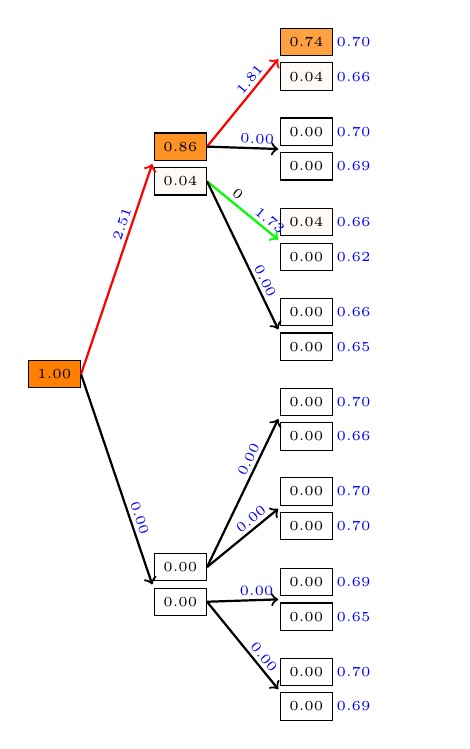
\begin{tikzpicture}
\tikzstyle{between} = [rectangle, minimum height=0.1cm, minimum width=0.70cm, draw opacity=0]
\tikzstyle{qval}    = [rectangle, text centered, text width=2cm]
\tikzstyle{qval}    = [rectangle, text centered, text width=2cm]
\node[between] at (-8.40, 2.67) (1_b_0){};
\node[between] at (-8.40, -2.67) (1_b_1){};
\node[between] at (-6.80, 4.00) (2_b_0){};
\node[between] at (-6.80, 2.86) (2_b_1){};
\node[between] at (-6.80, 1.71) (2_b_2){};
\node[between] at (-6.80, 0.57) (2_b_3){};
\node[between] at (-6.80, -0.57) (2_b_4){};
\node[between] at (-6.80, -1.71) (2_b_5){};
\node[between] at (-6.80, -2.86) (2_b_6){};
\node[between] at (-6.80, -4.00) (2_b_7){};
\node[rectangle, text centered, draw=black, minimum height=0.2cm, minimum width=0.45cm, fill=orange, fill opacity=1.00, draw opacity=1, text opacity=1] at (-10.00, 0.00) (0_s_0) {\tiny 1.00};
\node[rectangle, text centered, draw=black, minimum height=0.2cm, minimum width=0.45cm, fill=orange, fill opacity=0.86, draw opacity=1, text opacity=1] at (-8.40, 2.89) (1_s_0) {\tiny 0.86};
\node[rectangle, text centered, draw=black, minimum height=0.2cm, minimum width=0.45cm, fill=orange, fill opacity=0.04, draw opacity=1, text opacity=1] at (-8.40, 2.45) (1_s_1) {\tiny 0.04};
\node[rectangle, text centered, draw=black, minimum height=0.2cm, minimum width=0.45cm, fill=orange, fill opacity=0.00, draw opacity=1, text opacity=1] at (-8.40, -2.45) (1_s_2) {\tiny 0.00};
\node[rectangle, text centered, draw=black, minimum height=0.2cm, minimum width=0.45cm, fill=orange, fill opacity=0.00, draw opacity=1, text opacity=1] at (-8.40, -2.89) (1_s_3) {\tiny 0.00};
\node[rectangle, text centered, draw=black, minimum height=0.2cm, minimum width=0.45cm, fill=orange, fill opacity=0.74, draw opacity=1, text opacity=1] at (-6.80, 4.22) (2_s_0) {\tiny 0.74};
\node[qval] at (-6.20, 4.22) () {\tiny \textcolor{blue}{0.70}};
\node[rectangle, text centered, draw=black, minimum height=0.2cm, minimum width=0.45cm, fill=orange, fill opacity=0.04, draw opacity=1, text opacity=1] at (-6.80, 3.78) (2_s_1) {\tiny 0.04};
\node[qval] at (-6.20, 3.78) () {\tiny \textcolor{blue}{0.66}};
\node[rectangle, text centered, draw=black, minimum height=0.2cm, minimum width=0.45cm, fill=orange, fill opacity=0.00, draw opacity=1, text opacity=1] at (-6.80, 3.08) (2_s_2) {\tiny 0.00};
\node[qval] at (-6.20, 3.08) () {\tiny \textcolor{blue}{0.70}};
\node[rectangle, text centered, draw=black, minimum height=0.2cm, minimum width=0.45cm, fill=orange, fill opacity=0.00, draw opacity=1, text opacity=1] at (-6.80, 2.64) (2_s_3) {\tiny 0.00};
\node[qval] at (-6.20, 2.64) () {\tiny \textcolor{blue}{0.69}};
\node[rectangle, text centered, draw=black, minimum height=0.2cm, minimum width=0.45cm, fill=orange, fill opacity=0.04, draw opacity=1, text opacity=1] at (-6.80, 1.93) (2_s_4) {\tiny 0.04};
\node[qval] at (-6.20, 1.93) () {\tiny \textcolor{blue}{0.66}};
\node[rectangle, text centered, draw=black, minimum height=0.2cm, minimum width=0.45cm, fill=orange, fill opacity=0.00, draw opacity=1, text opacity=1] at (-6.80, 1.49) (2_s_5) {\tiny 0.00};
\node[qval] at (-6.20, 1.49) () {\tiny \textcolor{blue}{0.62}};
\node[rectangle, text centered, draw=black, minimum height=0.2cm, minimum width=0.45cm, fill=orange, fill opacity=0.00, draw opacity=1, text opacity=1] at (-6.80, 0.79) (2_s_6) {\tiny 0.00};
\node[qval] at (-6.20, 0.79) () {\tiny \textcolor{blue}{0.66}};
\node[rectangle, text centered, draw=black, minimum height=0.2cm, minimum width=0.45cm, fill=orange, fill opacity=0.00, draw opacity=1, text opacity=1] at (-6.80, 0.35) (2_s_7) {\tiny 0.00};
\node[qval] at (-6.20, 0.35) () {\tiny \textcolor{blue}{0.65}};
\node[rectangle, text centered, draw=black, minimum height=0.2cm, minimum width=0.45cm, fill=orange, fill opacity=0.00, draw opacity=1, text opacity=1] at (-6.80, -0.35) (2_s_8) {\tiny 0.00};
\node[qval] at (-6.20, -0.35) () {\tiny \textcolor{blue}{0.70}};
\node[rectangle, text centered, draw=black, minimum height=0.2cm, minimum width=0.45cm, fill=orange, fill opacity=0.00, draw opacity=1, text opacity=1] at (-6.80, -0.79) (2_s_9) {\tiny 0.00};
\node[qval] at (-6.20, -0.79) () {\tiny \textcolor{blue}{0.66}};
\node[rectangle, text centered, draw=black, minimum height=0.2cm, minimum width=0.45cm, fill=orange, fill opacity=0.00, draw opacity=1, text opacity=1] at (-6.80, -1.49) (2_s_10) {\tiny 0.00};
\node[qval] at (-6.20, -1.49) () {\tiny \textcolor{blue}{0.70}};
\node[rectangle, text centered, draw=black, minimum height=0.2cm, minimum width=0.45cm, fill=orange, fill opacity=0.00, draw opacity=1, text opacity=1] at (-6.80, -1.93) (2_s_11) {\tiny 0.00};
\node[qval] at (-6.20, -1.93) () {\tiny \textcolor{blue}{0.70}};
\node[rectangle, text centered, draw=black, minimum height=0.2cm, minimum width=0.45cm, fill=orange, fill opacity=0.00, draw opacity=1, text opacity=1] at (-6.80, -2.64) (2_s_12) {\tiny 0.00};
\node[qval] at (-6.20, -2.64) () {\tiny \textcolor{blue}{0.69}};
\node[rectangle, text centered, draw=black, minimum height=0.2cm, minimum width=0.45cm, fill=orange, fill opacity=0.00, draw opacity=1, text opacity=1] at (-6.80, -3.08) (2_s_13) {\tiny 0.00};
\node[qval] at (-6.20, -3.08) () {\tiny \textcolor{blue}{0.65}};
\node[rectangle, text centered, draw=black, minimum height=0.2cm, minimum width=0.45cm, fill=orange, fill opacity=0.00, draw opacity=1, text opacity=1] at (-6.80, -3.78) (2_s_14) {\tiny 0.00};
\node[qval] at (-6.20, -3.78) () {\tiny \textcolor{blue}{0.70}};
\node[rectangle, text centered, draw=black, minimum height=0.2cm, minimum width=0.45cm, fill=orange, fill opacity=0.00, draw opacity=1, text opacity=1] at (-6.80, -4.22) (2_s_15) {\tiny 0.00};
\node[qval] at (-6.20, -4.22) () {\tiny \textcolor{blue}{0.69}};
\draw[->, thick, red] (0_s_0.east) -- (1_b_0.west) node [pos=0.70, above=-0.2em, sloped, font=\tiny] () {\textcolor{blue}{2.51}};
\draw[->, thick, black] (0_s_0.east) -- (1_b_1.west) node [pos=0.70, above=-0.2em, sloped, font=\tiny] () {\textcolor{blue}{0.00}};
\draw[->, thick, red] (1_s_0.east) -- (2_b_0.west) node [pos=0.70, above=-0.2em, sloped, font=\tiny] () {\textcolor{blue}{1.81}};
\draw[->, thick, black] (1_s_0.east) -- (2_b_1.west) node [pos=0.70, above=-0.2em, sloped, font=\tiny] () {\textcolor{blue}{0.00}};
\draw[->, thick, green] (1_s_1.east) -- (2_b_2.west) node [pos=0.35, above=-0.2em, sloped, font=\tiny] () {\textcolor{black}{0}} node [pos=0.80, above=-0.2em, sloped, font=\tiny] () {\textcolor{blue}{1.73}};
\draw[->, thick, black] (1_s_1.east) -- (2_b_3.west) node [pos=0.70, above=-0.2em, sloped, font=\tiny] () {\textcolor{blue}{0.00}};
\draw[->, thick, black] (1_s_2.east) -- (2_b_4.west) node [pos=0.70, above=-0.2em, sloped, font=\tiny] () {\textcolor{blue}{0.00}};
\draw[->, thick, black] (1_s_2.east) -- (2_b_5.west) node [pos=0.70, above=-0.2em, sloped, font=\tiny] () {\textcolor{blue}{0.00}};
\draw[->, thick, black] (1_s_3.east) -- (2_b_6.west) node [pos=0.70, above=-0.2em, sloped, font=\tiny] () {\textcolor{blue}{0.00}};
\draw[->, thick, black] (1_s_3.east) -- (2_b_7.west) node [pos=0.70, above=-0.2em, sloped, font=\tiny] () {\textcolor{blue}{0.00}};
\end{tikzpicture}
\end{minipage}
\end{document}